
\chapter{Evaluation}

\section{Verifying Stack Protection}
% Create an example program. Show that accessing another task's stack memory yields fault.

\subsection{Reading/Writing Another Task's Stack}

\section{Verifying Heap Protection}
% Create an example program. Show that accessing another task's heap memory yields fault.

\subsection{Reading/Writing Another Task's Heap Memory}

\subsection{Freeing Another Task's Heap Memory}

\begin{figure}[h]
	\centering
	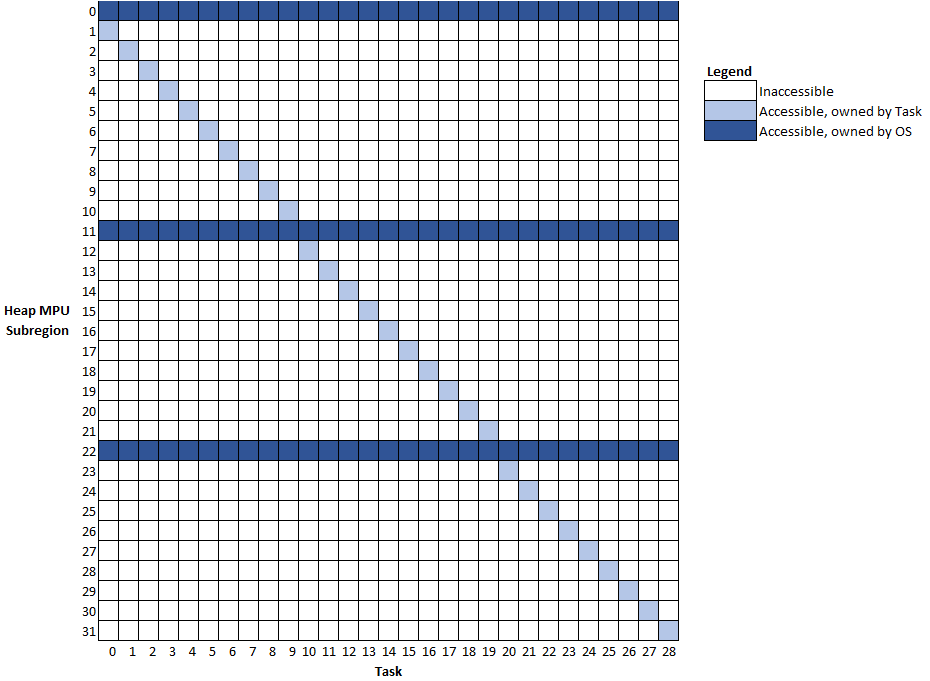
\includegraphics[width=\linewidth]{figs/task_access.png}
	\caption{Illustration of which tasks have access to which MPU subregions of the heap. This shows twenty-nine tasks, the maximum my solution can support with a 16KB heap.}
	\label{fig:task_access}
\end{figure}

Figure \ref{fig:task_access} shows which MPU subregions of the heap are accessible to which task for a system running twenty-nine tasks. One can see that all tasks can access OS subregions -- this is so that OS calls in the same privilege mode can touch OS data structures in the heap. Also, each task is allocated a unique subregion of its own, where its stack is located.

\section{Demonstrating Heap Flexibility}
% Show that my solution better handles dynamic memory use.

\section{Measuring Context Switch Overhead}

\begin{table}[h]
\centering
\begin{tabular}{|l|l|}
\hline
\textbf{Config}                                                                        & \textbf{Context Switch Time} \\ \hline
No Memory Protection                                                                   & 2.833 microseconds           \\ \hline
\begin{tabular}[c]{@{}l@{}}Memory Protection with\\ Heavy Reconfiguration\end{tabular} & 7.167 microseconds           \\ \hline
\begin{tabular}[c]{@{}l@{}}Memory Protection with\\ Lite Reconfiguration\end{tabular}  & 6.25 microseconds           \\ \hline
\end{tabular}
\caption{Context switch duration.}
\label{tab:ctxsw}
\end{table}

In Table \ref{tab:ctxsw}, I measure the context switch duration for no memory protection, memory protection with heavy reconfiguration, and my design: memory protection with lite reconfiguration. The implementation with heavy reconfiguration fully initializes each of the four MPU regions of the heap during each context switch. This approximates a solution in which each task and/or process in the system maintains its own set of MPU regions which must be programmed into the MPU prior to running. This is much ``heavier'' reconfiguration than merely masking subregions of a constant region configuration as in my solution. The addition of memory protection does lengthen the context switch duration. That said, the context switch is shorter than it would otherwise be thanks to the use of subregions, which enable relatively light reconfiguration of the MPU during a context switch compared to heavier approaches. Lite reconfiguration yields a reduction in context switch duration of 12.8\%.
